\chapter{Fast Data Migration}

In order to meet their latency and throughput goals, kernel-bypass
storage systems often start out with simple, stripped down designs with
the focus on fast, efficient request processing~\cite{mica}.
%
When it comes to distribution, hash partitioning is often the norm since
it is a simple, efficient, and scalable way of distributing load across
a cluster of machines.
%
Most systems tend to pre-partition records and tables into coarse hash
buckets, and then move these buckets around the cluster in response to
load imbalances~\cite{dynamo}.
%
However, coarse pre-partitioning can lead to high request fan-out when
applications exhibit temporal locality in the records they access,
hurting performance (Figure~\ref{fig:cluster-locality}) and cluster
utilization~\cite{rocksteady}.
%
Therefore, in order to be able to support a diverse set of applications
with different access patterns, these systems need to be more flexible
and lazy about how they partition and distribute data.

\begin{figure}[t]
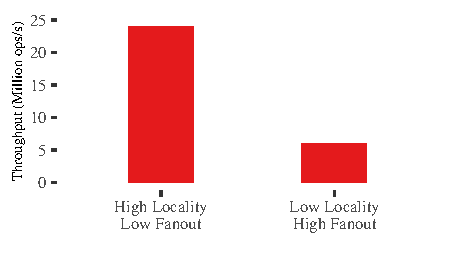
\includegraphics[width=\textwidth]{graphs/migration-motivation.pdf}
\caption{The impact of locality on cluster throughput. When locality is
low due to high fanout, a cluster of RAMCloud servers performs 6 Million
ops/s. On improving locality, by potentially migrating data to reduce
fanout, throughput improves to 24 Million ops/s}
\label{fig:cluster-locality}
\end{figure}


Flexible and lazy partitioning creates a unique challenge for
kernel-bypass storage systems.
%
Once a decision to partition is made, the partition must be quickly
moved to it’s new home with minimum impact to performance.
%
Doing so is hard; these
systems offer latencies as low as 5 microseconds,
so even a few cache misses will significantly hurt
performance.
%
Rocksteady~\cite{rocksteady} is a fast, low-impact
data migration protocol that tackles this problem.
%
Built on top of RAMCloud~\cite{ramcloud}, Rocksteady’s key insight is to
leverage application skew to speed up data migration while minimizing
the impact to performance.
%
When migrating a partition from a source to a target, it first migrates
ownership of the partition.
%
Doing so moves load on the partition from the source to the target, creating
headroom on the source that can be used to migrate data.
%
To keep the partition online, the target pulls records from the source
on-demand; since applications are skewed – most requests are for a small
set of hot records – this on-demand process converges quickly.

To fully utilize created headroom, Rocksteady carefully schedules and
pipelines data migration on both the source and target.
%
Migration is
broken up into tasks that work in parallel over RAMCloud’s hash table;
doing so keeps the pre-fetcher happy, improving cache locality.
%
A shared-memory model allows these tasks to be scheduled on any core,
allowing any idle compute on the source and target to be used for
migration.
%
To further speed up migration, Rocksteady delays
re-replication of migrated data at the target to until after migration
has completed.
%
Fault tolerance is guaranteed by maintaining a dependency
between the source and target at RAMCloud’s coordinator (called lineage)
during the migration, and recovering all data at the source if either
machine crashes.
%
Recovery must also include the target because of early
ownership transfer; the target could have served and replicated writes
on the partition since the migration began.
%
Putting all these parts
together results in a protocol that migrates data 100x faster than the
state-of-the-art while maintaining tail latencies 1000x lower.

Overall, Rocksteady’s careful attention to ownership, scheduling, and
fault tolerance allow it to quickly and safely migrate data with low
impact to performance.
%
Experiments show that it can migrate at 758 MBps
while maintaining tail latency below 250 microseconds; this is
equivalent to migrating 256 GB of data in 6 minutes, allowing for quick
scale-up and scale-down of a cluster.
%
Experiments also show the benefits
of leveraging skew: at low skew, Rocksteady keeps median latency below
75 microseconds, at high skew, it keeps median latency below 28
microseconds, and at even higher skew, Rocksteady keeps median latency
below 17 microseconds.
%
Additionally, early ownership transfer and
lineage help improve migration speed by 25\%.
%
These results have
important implications on system design; fast storage systems can use
Rocksteady as a mechanism to enable flexible, lazy partitioning of
data.
